\documentclass[border=8pt]{standalone}
% Shared preamble for IronClaw thesis figures (standalone TikZ).
\renewcommand{\familydefault}{\sfdefault}
\usepackage{tikz}
\usetikzlibrary{arrows.meta,positioning,calc,fit,backgrounds,shapes.geometric,shapes.misc}

% IronClaw palette (matches slides.tex)
\definecolor{IronDark}{HTML}{1A2B3C}
\definecolor{IronBlue}{HTML}{2E86AB}
\definecolor{IronTeal}{HTML}{06A77D}
\definecolor{IronOrange}{HTML}{F18F01}
\definecolor{IronRed}{HTML}{C73E1D}
\definecolor{IronLight}{HTML}{F4F7F9}
\definecolor{IronGray}{HTML}{5D6D7E}

\tikzset{
  figtitle/.style={font=\large\bfseries\color{IronDark}, align=center},
  hostbox/.style={draw=IronBlue, rounded corners=5pt, fill=IronBlue!8,
                  line width=1pt, align=center, font=\small\color{white}},
  hostfill/.style={draw=IronBlue, rounded corners=4pt, fill=IronBlue,
                   line width=0.8pt, align=center, font=\small\color{white},
                   text width=3.1cm, minimum height=0.85cm},
  guestfill/.style={draw=IronOrange, rounded corners=4pt, fill=IronOrange!85,
                    line width=0.8pt, align=center, font=\small\color{white},
                    text width=3.1cm, minimum height=0.85cm},
  guestsoft/.style={draw=IronOrange, rounded corners=4pt, fill=IronOrange!25,
                    line width=0.8pt, align=center, font=\small\color{IronDark},
                    text width=3.1cm, minimum height=0.75cm},
  arrow/.style={-{Latex[length=2.6mm,width=2mm]}, line width=0.9pt, IronDark},
  biarrow/.style={{Latex[length=2.6mm,width=2mm]}-{Latex[length=2.6mm,width=2mm]},
                  line width=0.9pt, IronDark},
  note/.style={font=\footnotesize\color{IronGray}, align=center},
}

\begin{document}
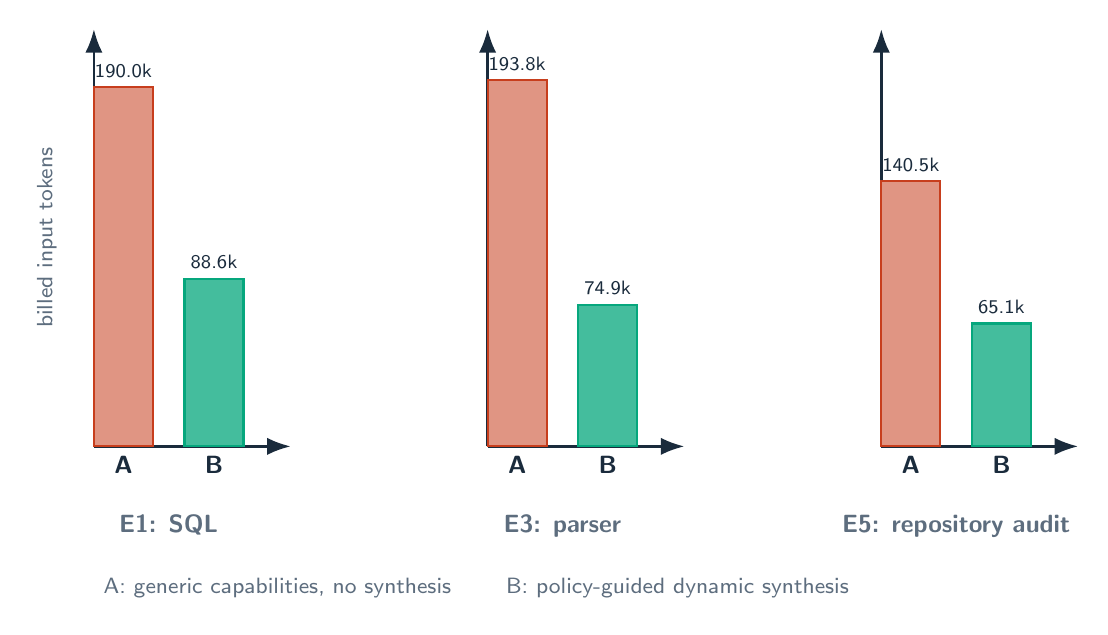
\begin{tikzpicture}
  \tikzset{
    bar/.style={line width=0.8pt, minimum width=0.75cm},
    axis/.style={-{Latex[length=3mm,width=2.2mm]}, line width=1pt, IronDark},
    barlabel/.style={font=\scriptsize\color{IronDark}, align=center},
    scenlabel/.style={font=\small\bfseries\color{IronDark}, align=center},
    paneltitle/.style={font=\small\bfseries\color{IronGray}, align=center},
  }

  % scale: 0.024 cm per 1k input tokens
  \begin{scope}
    \draw[axis] (0,0) -- (2.5,0);
    \draw[axis] (0,0) -- (0,5.3);
    \node[note, rotate=90, anchor=south] at (-0.35,2.65) {billed input tokens};
    \filldraw[bar, draw=IronRed, fill=IronRed!55] (0.00,0) rectangle (0.75,4.56);
    \filldraw[bar, draw=IronTeal, fill=IronTeal!75] (1.15,0) rectangle (1.90,2.13);
    \node[barlabel, anchor=south] at (0.375,4.56) {190.0k};
    \node[barlabel, anchor=south] at (1.525,2.13) {88.6k};
    \node[scenlabel, anchor=north] at (0.375,0) {A};
    \node[scenlabel, anchor=north] at (1.525,0) {B};
    \node[paneltitle, anchor=north] at (0.95,-0.75) {E1: SQL};
  \end{scope}

  \begin{scope}[xshift=5.0cm]
    \draw[axis] (0,0) -- (2.5,0);
    \draw[axis] (0,0) -- (0,5.3);
    \filldraw[bar, draw=IronRed, fill=IronRed!55] (0.00,0) rectangle (0.75,4.65);
    \filldraw[bar, draw=IronTeal, fill=IronTeal!75] (1.15,0) rectangle (1.90,1.80);
    \node[barlabel, anchor=south] at (0.375,4.65) {193.8k};
    \node[barlabel, anchor=south] at (1.525,1.80) {74.9k};
    \node[scenlabel, anchor=north] at (0.375,0) {A};
    \node[scenlabel, anchor=north] at (1.525,0) {B};
    \node[paneltitle, anchor=north] at (0.95,-0.75) {E3: parser};
  \end{scope}

  \begin{scope}[xshift=10.0cm]
    \draw[axis] (0,0) -- (2.5,0);
    \draw[axis] (0,0) -- (0,5.3);
    \filldraw[bar, draw=IronRed, fill=IronRed!55] (0.00,0) rectangle (0.75,3.37);
    \filldraw[bar, draw=IronTeal, fill=IronTeal!75] (1.15,0) rectangle (1.90,1.56);
    \node[barlabel, anchor=south] at (0.375,3.37) {140.5k};
    \node[barlabel, anchor=south] at (1.525,1.56) {65.1k};
    \node[scenlabel, anchor=north] at (0.375,0) {A};
    \node[scenlabel, anchor=north] at (1.525,0) {B};
    \node[paneltitle, anchor=north] at (0.95,-0.75) {E5: repository audit};
  \end{scope}

  \node[note, anchor=west] at (0,-1.8)
    {A: generic capabilities, no synthesis \qquad B: policy-guided dynamic synthesis};
\end{tikzpicture}
\end{document}
